\chapter{Materials and methods}
\label{Chap3}
\section{Powder follow-up}

\subsection{Sieving}

\subsection{Grain size and distribution}

\subsection{Composition}

%\subsection{Drying}

\section{SLM manufacturing}
\label{MMFPP}
The same direct metal printer (DMP) was used to fabricate all specimens throughout this work. It is a \textit{ProX DMP 200} printer, manufactured by \textit{3D Systems} (see figure \ref{fig:Printer}). It uses a laser with a theoretical maximal power of 300 [W] and wavelength $\lambda$ = 1070 [nm] \parencite{3D}. Its actual maximal power is $P_{max}=273.6 [W]$. \textcolor{gray}{[QUEL EST LE SPOT SIZE?]}  The maximal envelope capacity of the machine (W x D x H) is 140 x 140 x 125 [mm]. Its typical accuracy is +/- 50 [$\mu m$] for small parts and +/- 0.2\% for large parts. It allows for the set-up of a protection atmosphere. However, it does not integrate any heating feature for the build bed.\\

\begin{figure}[ht]
\centering
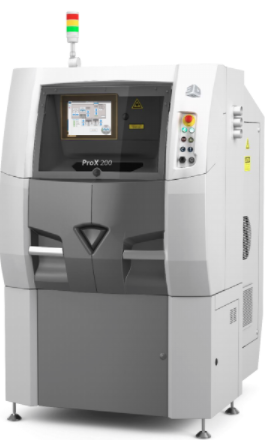
\includegraphics[scale=0.7]{Images/Printer}
\decoRule
\caption[ProX DMP 200 printer]{ProX DMP 200 printer (from the user's ProX DMP 200 general instructions document).}
\label{fig:Printer}
\end{figure}

In this thesis, argon was used as shielding gas. The composition of the gas environment was monitored so as to keep $p_{O2}$ < 500 [ppm]. Laser compensations were set to take into account the excess energy at the start and end of the scanning vectors (see figure \ref{fig:Compens}). These were chosen in accordance with the manufacturer recommendations (figure \ref{fig:Compens1}). Values for hatch space (h) and layer thickness (t) were respectively set to 100 [$\mu m$] and 30 [$\mu m$]. The scan speed ($v_s$) and the laser power (P) were varied in the ranges [900 ; 1500] [$\frac{mm}{s}$] and [$0.75 \cdot P_{max}$ ; $P_{max}$] respectively, in order to optimise of the built specimens (see section \ref{Rparaopti}). Educated guesses were made based on literature and previous works done at the UCL. The parameters used are resumed in appendix \ref{ppa}. Batches were named in the format X200-\textit{yymmdd}. The prefix "X200" refers to the DMP used. It is followed by the date of printing (6 digits). Recycled powder was used for every batch except for X200-180222 and X200-180228. Figures with detailed specimens positions, denominations, scanning orders and sintering durations for all batches are available in appendix \ref{mda}.\\

\begin{figure}[ht]
\centering
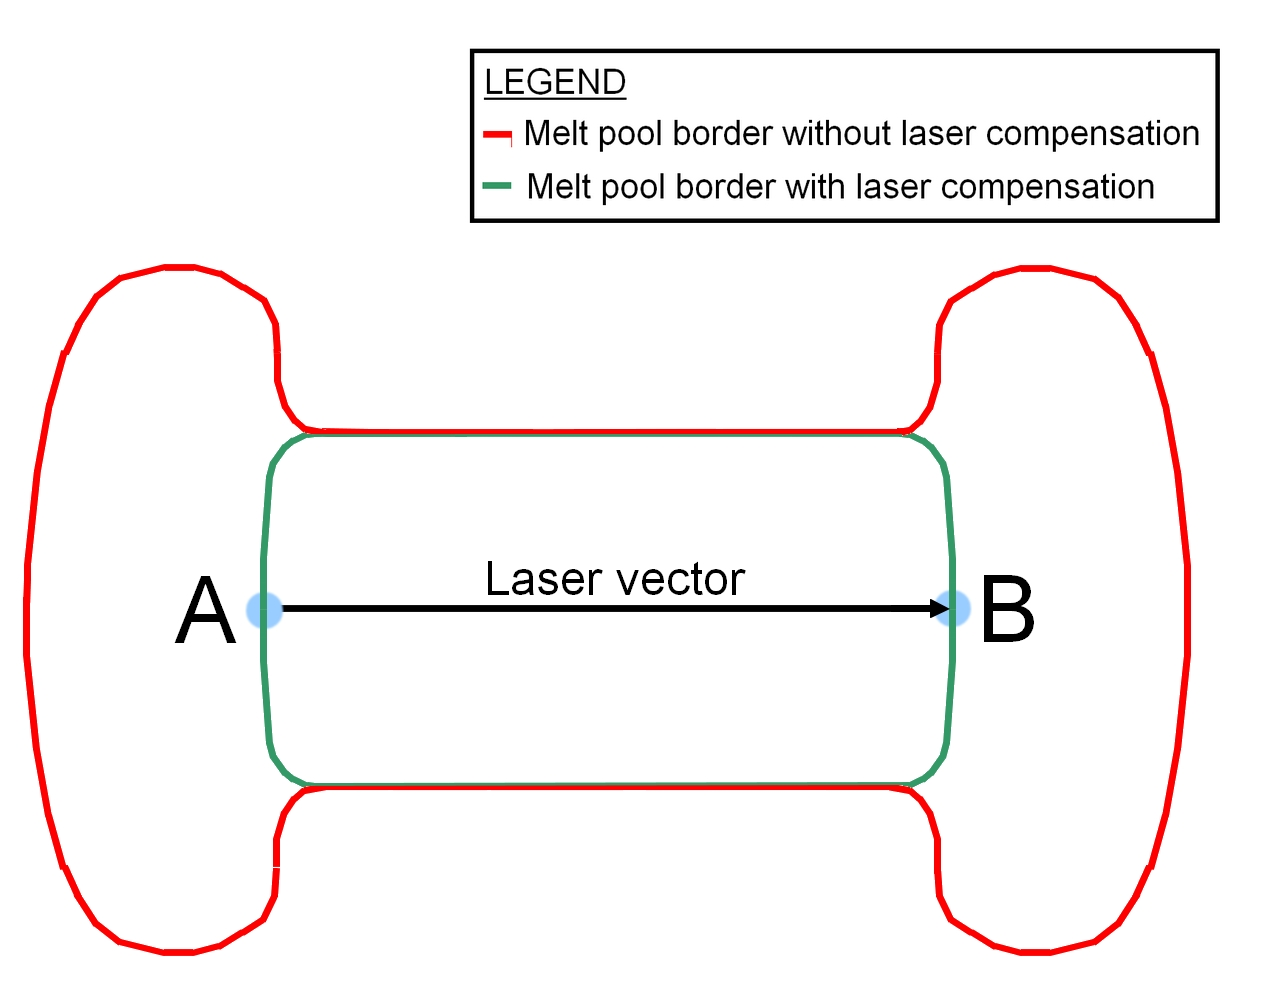
\includegraphics[scale=0.3]{Images/Compens}
\decoRule
\caption[Melt pool contours with and without laser compensation (exaggeration)]{Melt pool contours with and without laser compensation (exaggeration).}
\label{fig:Compens}
\end{figure}

\begin{figure}[ht]
\centering
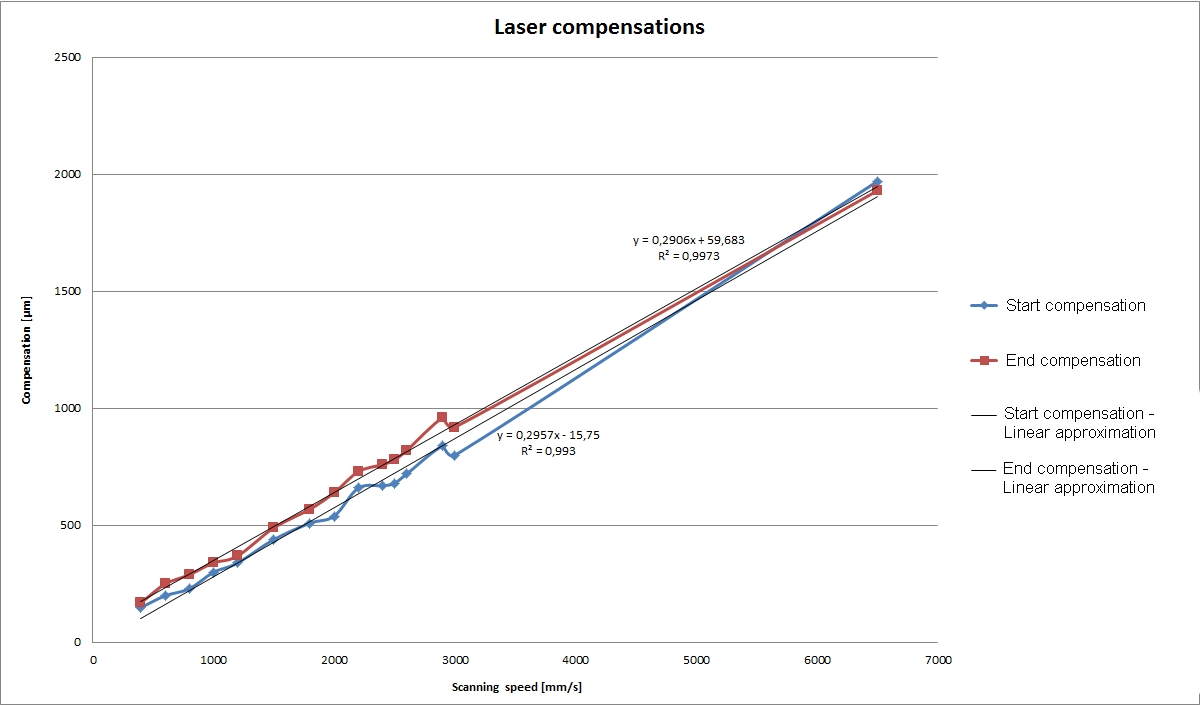
\includegraphics[scale=0.45]{Images/Compens1}
\decoRule
\caption[Laser compensations as a function of the scanning speed (as recommended by the manufacturer)]{Laser compensations as a function of the scanning speed (as recommended by the manufacturer).}
\label{fig:Compens1}
\end{figure}

The batches were first prepared on \textit{DMP ProX Manufacturing}, a dedicated CAD software. It enabled to select the values for the parameters previously mentioned, as well as the position of the specimens. Each specimen was fabricated on building supports. After the completion of the process, they were separated from the plate through electro-erosion. \\

For this thesis, all cylinders and tensile specimens were fabricated vertically. The dimensions notations for the samples types and the tensile specimens detailed geometry are gathered on figure \ref{fig:cc}.\\

\begin{figure}[ht]
\centering
\noindent\makebox[\textwidth]{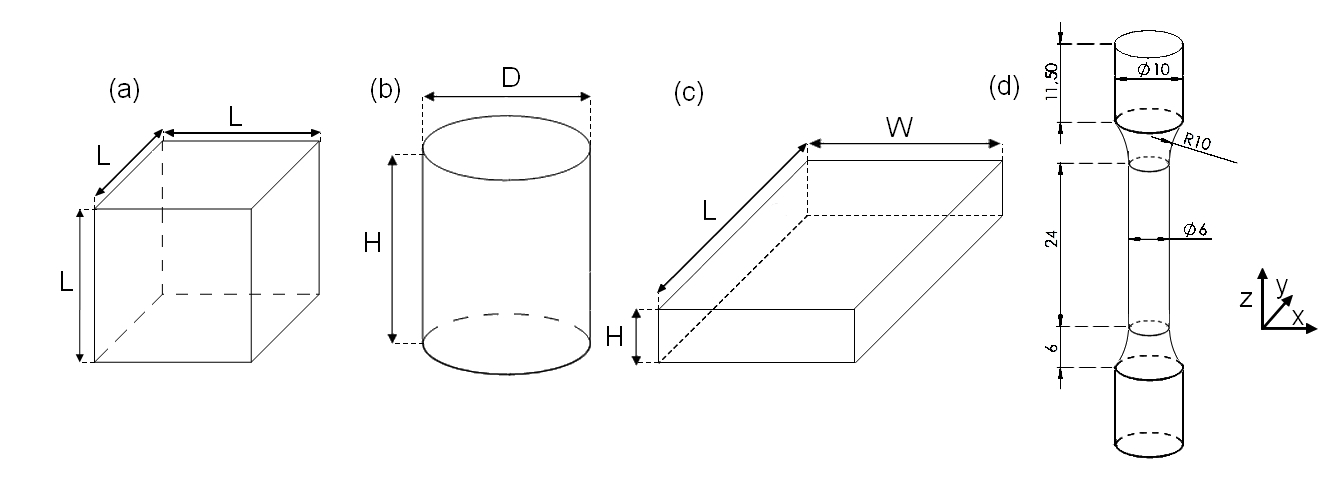
\includegraphics[scale=0.52]{Images/cc}}
\decoRule
\caption[Dimensions notations for (a) cubic specimens (b) cylindrical specimens (c) parallelepiped specimens (d) tensile specimen]{Dimensions notations for (a) cubic specimens (b) cylindrical specimens (c) parallelepiped specimens (d) tensile specimens with dimensions in [mm]}
\label{fig:cc}
\end{figure}


An island scanning strategy was chosen on account of research done on the subject (see section \ref{pp}). It is a hexagonal pattern. The replicated hexagon's smallest width is equal to 5 [mm]. An overlap of 100 [$\mu m$] was set, as illustrated on figure \ref{fig:OL}. There is a rotation of $90^\circ$ and a translation of a third of basis vector between two successive powder layers as depicted by figure \ref{fig:Lassup}. In the case of a contour scanning strategy, the contours were pre scanned for each powder layer with the same P and $v_s$ used for the bulk (see figure \ref{fig:LasCSC}). The scanning order among the samples was automatically chosen. \\

\begin{figure}[ht]
\centering
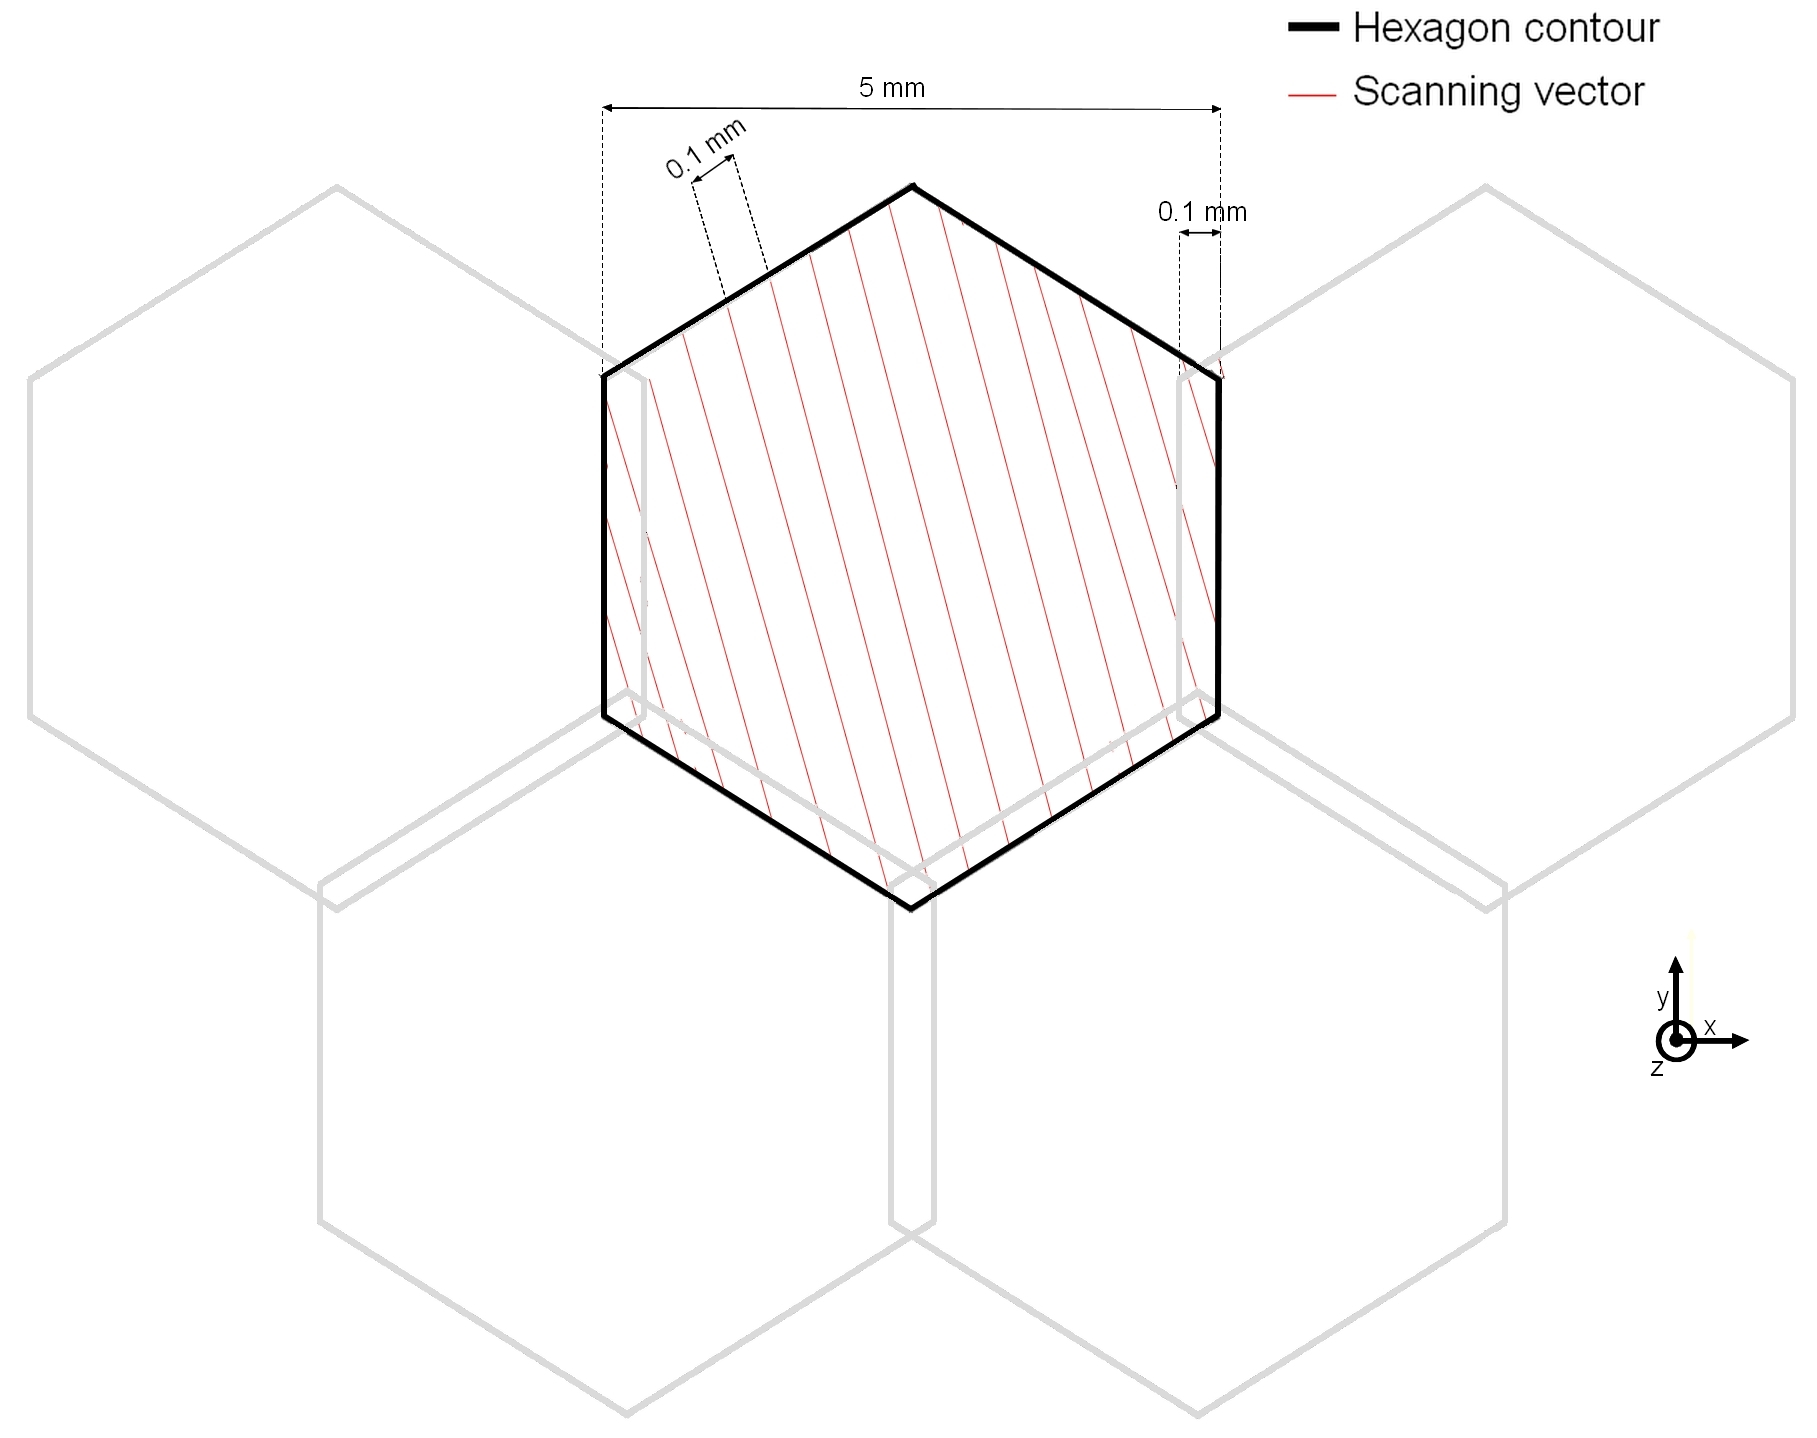
\includegraphics[scale=0.27]{Images/OL}
\decoRule
\caption[Schematic representation of the hexagonal pattern scanning strategy]{Schematic representation of the hexagonal pattern scanning strategy}
\label{fig:OL}
\end{figure}

\begin{figure}[ht]
\centering
\noindent\makebox[\textwidth]{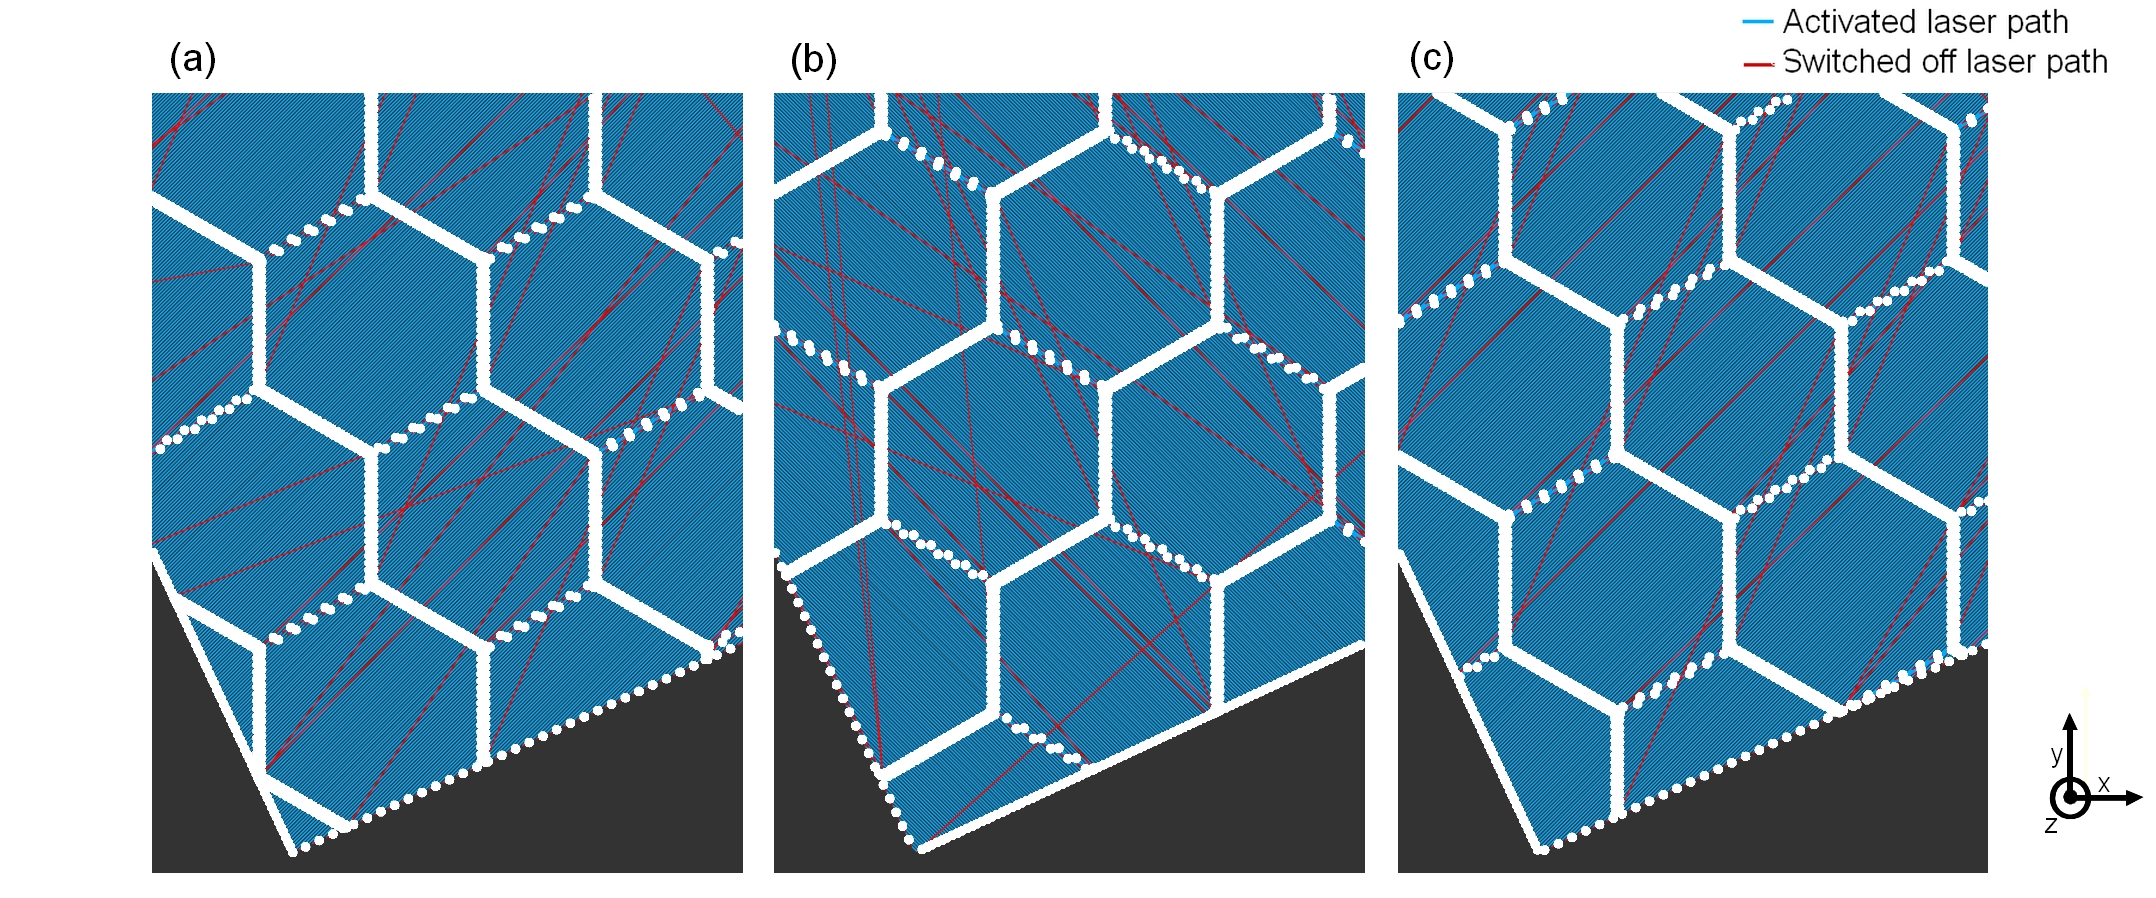
\includegraphics[scale=0.3]{Images/Lassup}}
\decoRule
\caption[Screen capture of the laser scanning pattern for a parallelepiped sample: (a) Layer $n$ (b) Layer $n+1$ (c) Layer $n+2$]{Laser scanning pattern for a parallelepiped sample: (a) Layer $n$ (b) Layer $n+1$ (c) Layer $n+2$}
\label{fig:Lassup}
\end{figure}

\begin{figure}[ht]
\centering
\noindent\makebox[\textwidth]{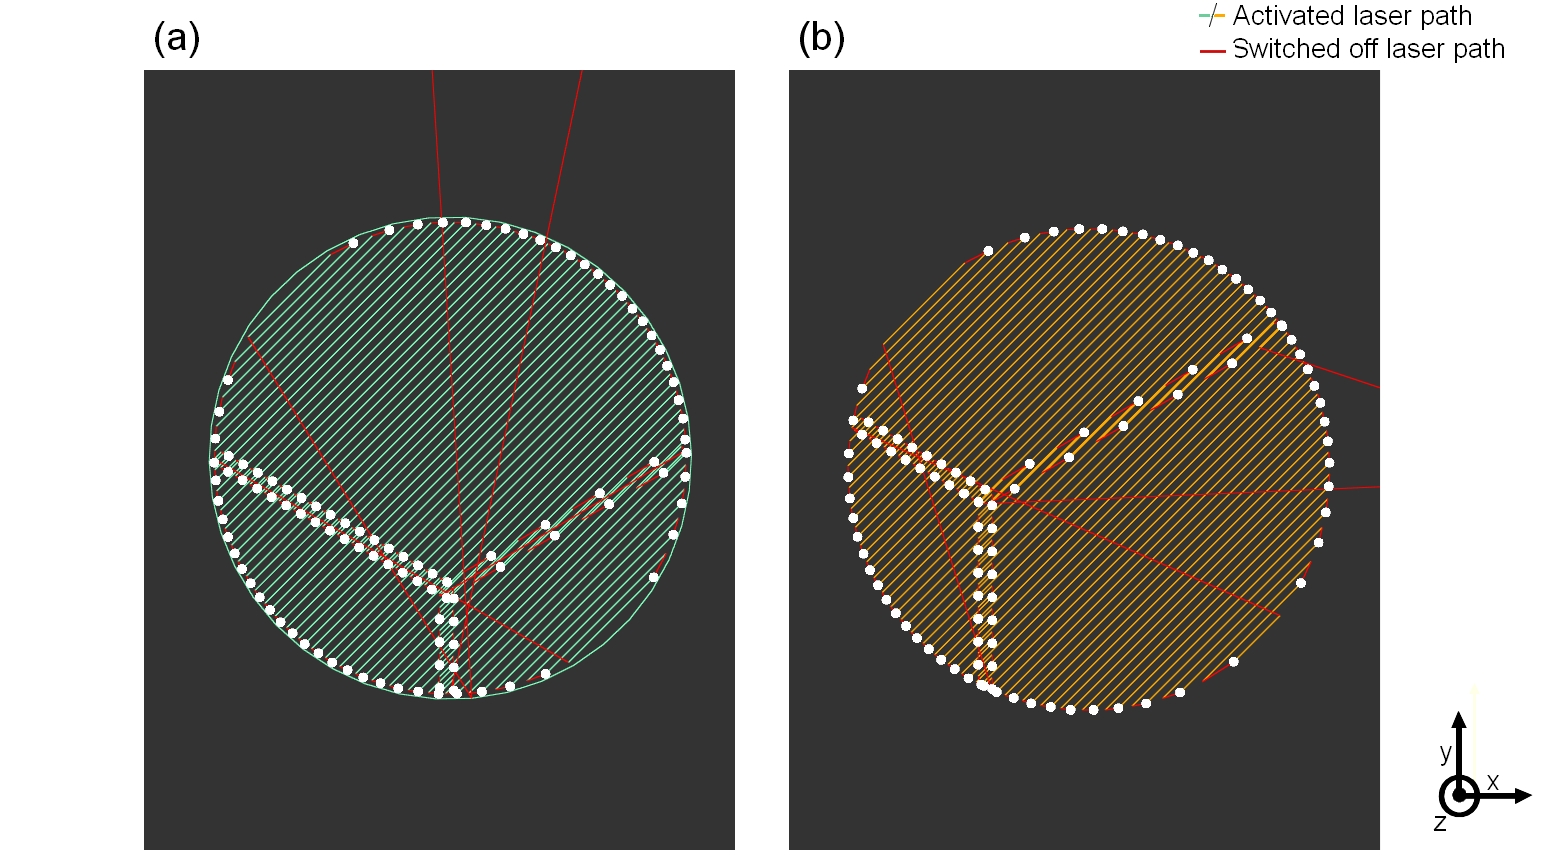
\includegraphics[scale=0.4]{Images/LasCSC}}
\decoRule
\caption[Screen capture of the laser path for a cylindric sample (a) with contour scanning strategy (b) without contour scanning strategy]{Screen capture of the laser path for a cylindric sample (a) with contour scanning strategy (b) without contour scanning strategy}
\label{fig:LasCSC}
\end{figure}
\section{Heat treatments}
\label{MMHT}
The heat treatments were conducted inside a unique oven of the VT 5050 EKP model, manufactured by Heraeus, which is able to reach a temperature of 400$^\circ$ C. Samples temperature data was obtained through a thermocouple welded to the sample surface, thanks to a ... . \textcolor{gray}{[Méthode de soudage, élévation de la température durant l'opération]} The data was displayed and saved every 10 seconds, with a precision of 0.1$^\circ$ C, thanks to a Agilent 34972A LXI Data Acquisition/Switching Unit, connected to the thermocouple (see Fig. for both devices). For unknown reasons, that can not be explained only by thermal inertia, setting the oven to the target temperature proved unable to heat the specimens to the same temperature. After a couple samples for testing, the method applied for following ones was to set the oven at a temperature about 20$^\circ$ C above the target, so that the data acquisition unit connected to the thermocouple displays the right temperature.\\

Due to the inaccuracy of the oven, maintaining the samples at the exact target temperature has not proved possible. The holding plateaus were thus rather slow increasing slopes. For most of the samples, the theoretical beginning of the holding was set when the specimen reached a temperature 5$^\circ$ C below the target value, so that the sample average temperature for the complete holding was the closest possible to target value.\\

Samples that were subject to a heat treatment were named in a particular format, to ease distinction between them. They received the name of the batch, followed by "TT-\textit{holdingtemperature-holdingtime-specificities}". Cubes that were subject to heat treatments were 5 x 5 x 5 [mm$^3$].\\

%\begin{figure}[ht]
%	\centering
%	\includegraphics[scale=0.7]{Images/HTdevices}
%	\decoRule
%	\caption[ProX DMP 200 printer]{ProX DMP 200 printer (from the user's ProX DMP 200 general instructions document).}
%	\label{fig:HTdevices}
%\end{figure}

The main objective of most of the research about aluminium alloys AM is to obtain parts with properties at least as good as their conventional cast counterparts. To obtain a larger panel of properties, a vast number of heat treatments have been developed for die cast alloys. The classical treatment of stress-relief for aluminium consists of a heating up to 300$^\circ$ C, with a holding of 2 hours, followed by a slow cooling\ref{label}. This treatment, and variations around him, have been tried on a number of additively manufactured samples, in order to assess their effect on the microstructure and mechanical properties of the parts.\\

A first series of cubic samples was manufactured using the optimised process parameters from Section \ref{Rparaopti}, and a different heat treatment was applied to each one of them. The complete list of cubes treated can be found in Table \ref{RTT}.\\

\begin{center}
\begin{table}[ht]
\noindent\makebox[\textwidth]{\begin{tabular}{|c|c|c|c|}
	\hline 
	Specimen & Holding time [min] & Aimed holding temp. [$^\circ$C] & Max. temp. [$^\circ$C] \\ 
	\hline 
	X200-180220-TT150-2 & 120 & 150 & - \\ 
	\hline 
	X200-180220-TT200-2 & 120 & 200 & - \\ 
	\hline 
	X200-180220-TT300-2 & 120 & 300 & 256 \\ 
	\hline 
	X200-180220-TT300-2-plaque & 120 & 300 & 281 \\ 
	\hline 
	X200-180220-TT150-2-real & 120 & 150 & 156 \\ 
	\hline 
	X200-180220-TT200-2-real & 120 &200  & 203 \\ 
	\hline 
	X200-180220-TT250-2-real & 120 & 250 & 255 \\ 
	\hline 
	X200-180220-TT300-2-real & 120 & 300 & 302 \\ 
	\hline 
	X200-180220-TT300-1-real & 60 & 300 & 302 \\ 
	\hline 
	X200-180220-TT360-1-real & 60 & 360 & 371 \\ 
	\hline 
	X200-180220-TT300-5m & 5 & 300 & 300 \\ 
	\hline 
\end{tabular}} 

\caption[List of the heat-treated specimens from batch X200-180220]{List of the heat-treated specimens from batch X200-180220}
\label{tab:RTT}
\end{table}
\end{center}


\section{Characterisation}

\subsection{Density}

\subsubsection{Hydrostatic weighing}

Multiple methods were considered to estimate the relative density of the fabricated specimens. The first one is hydrostatic weighting (HW), or hydrodensitometry. It is a direct application of the well-known Archimedes' principle, which can be stated as follows: " When a body is (partially or totally) immersed in a fluid, the upthrust on the body is equal to the weight of fluid displaced." \parencite{ADictionaryofPhysics}. By weighing each pieces in air and in water - giving respectively values of dry weight $W_a$ and underwater weight $W_w$ - one can calculate the apparent density $\rho_a$ \parencite{MethArch}:

$$\rho_a=\frac{W_a}{W_a-W_w} \cdot \rho_w $$

where $\rho_w$ is the water density. The apparent relative density $\rho_{a,rel}$ of the specimens can then be calculated with:

$$\rho_{a,rel} = \frac{\rho_a}{\rho_b} $$

where $\rho_b = 2.68 [\frac{g}{mm^3}]$ is the theoretical bulk density of AlSi10Mg \parencite{Bulk}. All weightings were done with a \textit{Sartorius BP121S} analytical balance with precision of 0.1 [mg] \parencite{Balance}. Samples were immersed in demineralised water for more than twelve hours before the measurements to impregnate them. The weightings were also done in demineralised water. Water temperature was measured with a precision glass thermometer to compute $\rho_w$ as accurately as possible thanks to tabulated values \parencite{Eau}. Multiple measurements were done for each sample in order to increase the method's reliability. \\

The technique was employed with "as-built" and polished cubes. For this second option, all six faces of the tested cubes were polished with P320 silicon carbide sandpaper sheets and briefly with P1200 ones. In most cases, the tests were done with samples of volumes $\simeq 1 [cm^3]$ and weights $\simeq 2.5 [g]$.\\

\subsubsection{Relative optical density image analysis}

Another method was used to estimate the relative density of the various samples: the relative optical density image analysis (RODIA). For this purpose, the samples were cut with a micro-cutting machine and underwent the polishing routine detailed in table \ref{tab:pol}. Pictures of the polished sections were then taken under the optical microscope. An \textit{Olympus AX70} microscope was used, with 5x and 10x magnification. The pictures were taken with a smart-phone through the lens of the microscope. The used camera has a resolution of 16 [MP]. A camera is directly connected to the microscope at the laboratory, but it only has 5 [MP] resolution. It was thus chosen not to use it. \\

With the help of the \textit{ImageJ} software, the surface of both the porosities and the whole surface could be isolated for each analysed image (see figure \ref{fig:ImageJ}). The surface fraction occupied by porosities could then be obtained as the ratio between the areas of the two (in pixels). If we approximate that the porosities surface fraction is equal to the volumetric one, that method gives an estimation of the relative density $\rho_{rel}$.

\begin{center}
\begin{table}[ht]
\noindent\makebox[\textwidth]{\begin{tabular}{|c|c |c |c| c|c|}
    \hline
    Step &  Polishing surface & Abrasive & Grain size & Lubricant type & Rotation speed [rpm]\\

\hline
\hline   
    1 & MD-piano 220 & Diamond & P220 & Water & 200-300 \\
    2 & MD-piano 1200 & Diamond & P1200 & Water & 200-300\\
    3 & MD-largo & DP-spray & 9 $\mu m$ & Alcohol & 150\\    
    4 & DP-DAC & DP-spray & 3 $\mu m$ & Alcohol & 150 \\ 
    5 & DP-NAP & DP-spray & 1 $\mu m$ & Alcohol & 150 \\  
    \hline

\end{tabular}}

\caption[Polishing routine for Al-Si alloys]{Polishing routine for Al-Si alloys}
\label{tab:pol}
\end{table}
\end{center}

\begin{figure}[ht]
\centering
\centerline{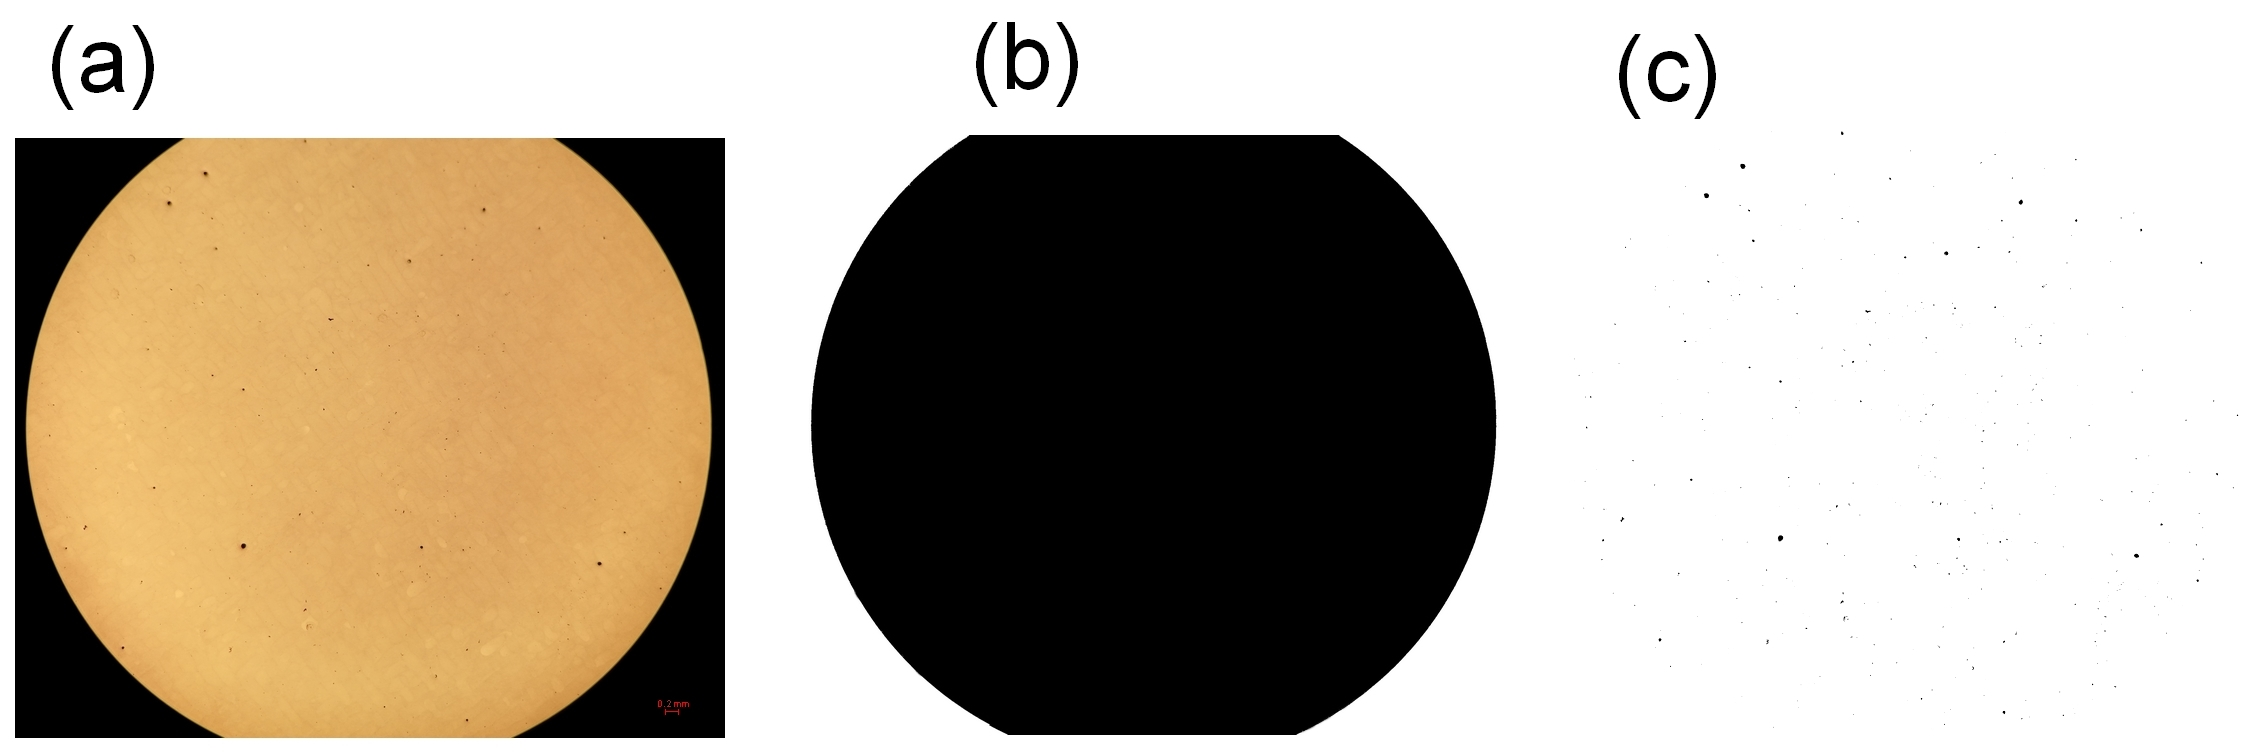
\includegraphics[scale=0.29]{Images/ImageJ-cub1}}
\decoRule
\caption[RODIA procedure for specimen X200-180319-cub 1: (a) Original picture of polished section (b) Whole surface isolation with \textit{ImageJ} (c) Porosities isolation with \textit{ImageJ}.]{RODIA procedure for specimen X200-180319-cub 1: (a) Original picture of polished section (b) Whole surface isolation with \textit{ImageJ} (c) Porosities isolation with \textit{ImageJ}.}
\label{fig:ImageJ}
\end{figure}

The images isolations in "foregrounds" and "backgrounds" were done through manual thresholding based on pixel intensity quantifications.  %https://imagej.net/Thresholding#Global_thresholding
An optimal threshold was sought for porosities isolation so as to include only holes, and as many as possible. Particular attention was given to the photography in order to obtain the best contrast, focus and intensity homogeneity. Between two and five photographs were taken for each specimen to build a representative sample.

\subsection{Microstructure}

\subsubsection{Scanning electron microscopy}

\subsubsection{Optical microscopy}
\label{MMOM}
Mesures Taille de bains:


In order to make the identification of the melt pools boundaries possible, the samples underwent the polishing routine detailed in table \ref{tab:pol}. They were then etched with	a Keller's reagent. It is a popular etchant containing hydrochloric acid, hydrofluoric acid and nitric acid diluted in distilled water. [Attaque préférentielle->distinction à l'optique][ + ImageJ] As SLM involves melt pools overlapping to ensure consolidation, one cannot measure the actual original melt pools dimensions. The method has thus only been used   as a tool to compare samples.

Densité
Autre chose?
\subsection{Composition}

\subsection{Residual stresses}

Measurements of residuals stresses was performed by ..., in ..., Malta. Four parallelepiped specimens were specifically built for these tests. Their dimensions was x  x  x [mm$^3$]. After undergoing their heat treatments, they were machined \textcolor{gray}{électro-découpage}, removing the least matter possible, and shipped to Malta. Machining was done in order to reduce rugosity on the top and bottom faces of the samples, because smooth surfaces are necessary for the correct fixation of the probes. \\

\subsection{Mechanical properties}

\subsubsection{Hardness test}

Vickers hardness measurements were made with a \textit{Wolpert Dia-Testor 2RC} tester. All analysed specimens were previously cut with a micro-cutting machine. This permitted the testing of the bulk hardnesses of the samples (at least at a few millimetres from the original surfaces). For each test, a pyramidal indenter (see figure \ref{fig:Vick}) was pressed during 10 [sec] onto the material with a load of 10 [kg]. The indentation durations were measured with a digital timer and the tests were stopped manually. The two diagonals lengths of the resulting indents were then evaluated using a ruler on the screen of the machine, which displays the image of the sample's surface that is captured by an embedded optical microscope.\\

\begin{figure}[ht]
\centering
\centerline{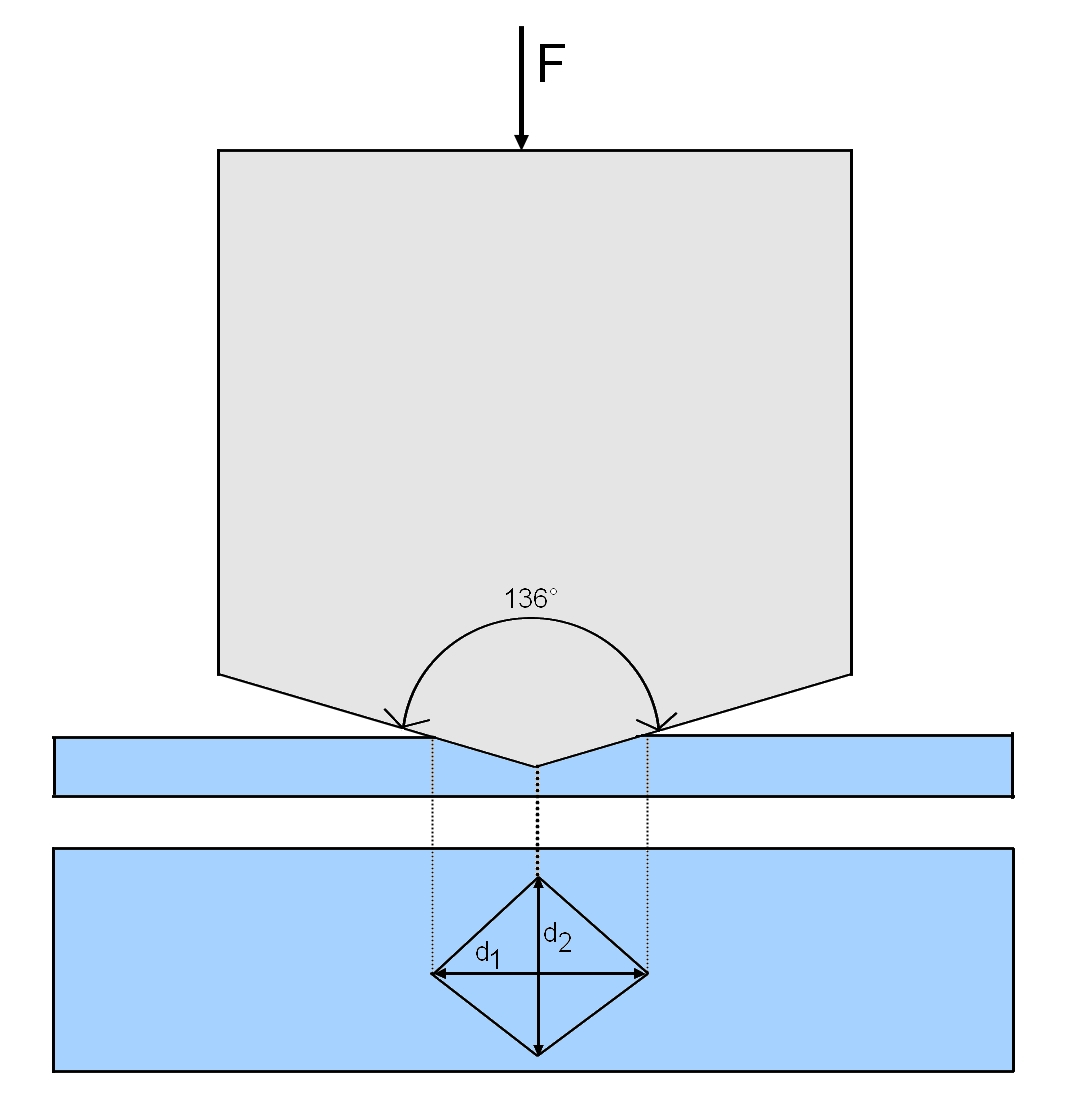
\includegraphics[scale=0.29]{Images/Vickers}}
\decoRule
\caption[Schematic representation of the Vickers hardness test]{Schematic representation of the Vickers hardness test}
\label{fig:Vick}
\end{figure}

Three to ten tests were made for each sample and the mean diagonal length value was computed for every test. The corresponding Vickers hardness values $H_v$ could then be estimated by means of a conversion table (see \ref{AppendixB}).\\

\subsubsection{Tensile tests}
\label{MMTT}
The tensile tests were performed on a \textit{RetroLine testControl II} screw-driven electro-mechanical testing system manufactured by \textit{Zwick Roell}. It works in the following manner:

\begin{itemize}
\item The cylindrical specimen is clamped on its extremities with grips. Both of them are fixed to a cross head (see figure \ref{fig:Trac}).

\item Parameters are selected thanks to a software connected to the machine: 
One must enter the extensometer initial gauge length $L_0$, the cross head speed and the pre load (used to limit the backlash in the assembly). The initial minimal value $d_o$ for the specimen diameter is also measured with a digital calliper and specified in the program.

\item The contact extensometer is placed on the sample. Its purpose is to measure the length change $\Delta L$ during the test. 

\item The lower cross head goes down. This induces a force $F$ and a displacement in the specimen, both of which are saved in an \textit{Excel} file. The test goes on until the fracture of the specimen occurs, unless if it is stopped beforehand.
\end{itemize}

\begin{figure}[ht]
\centering
\centerline{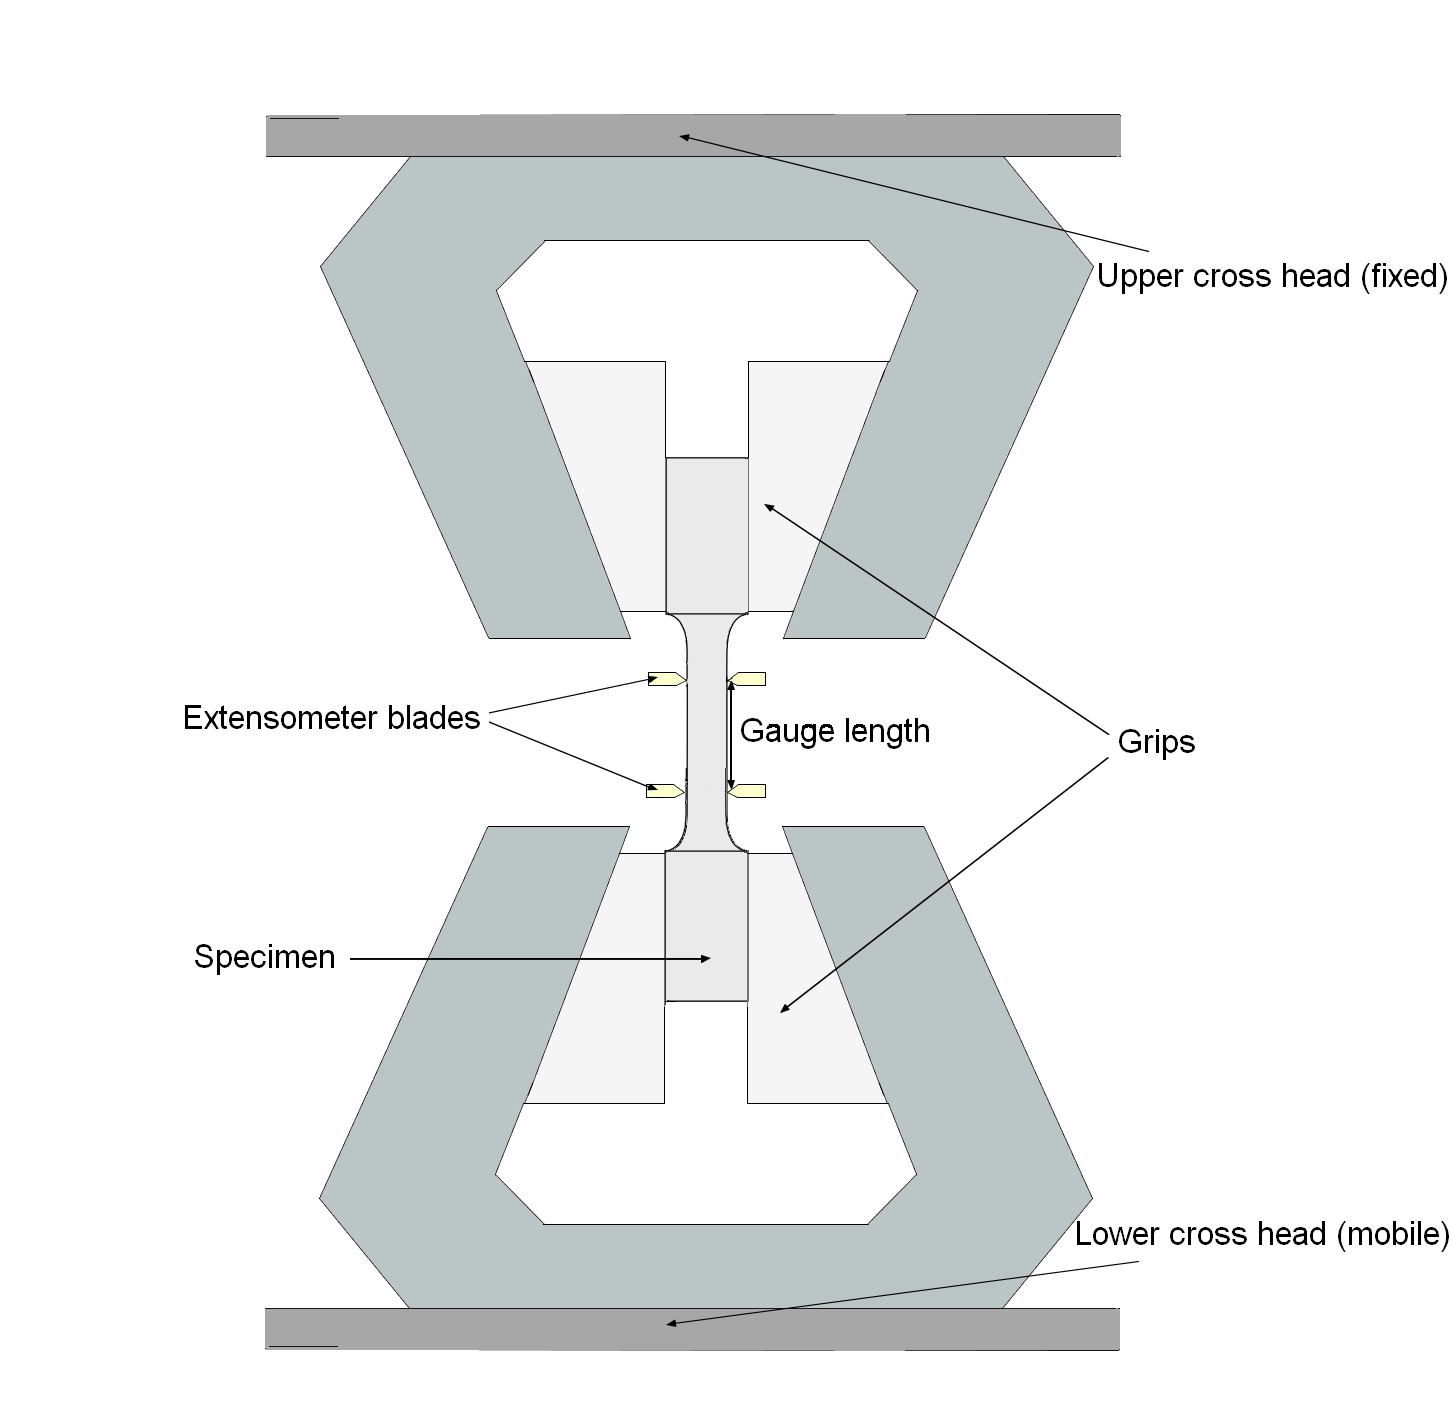
\includegraphics[scale=0.3]{Images/Trac}}
\decoRule
\caption[Schematic representation of the tensile test mounting]{Schematic representation of the tensile test mounting}
\label{fig:Trac}
\end{figure}

The tensile specimens used all originated from batch X200-190417. They were fabricated using the optimised set of parameters: $P=0.75\% P_{max}$ and $v_s=1200 [\frac{mm}{s}]$. Their minimal diameter is equal to 6 [mm]. Further details about their geometry and heat treatments can be consulted respectively in sections \ref{MMFPP} and \ref{MMHT}. For each test, the extensometer gauge length was set to 18 [mm]. This is approximately the maximal possible value, given the short length of the specimens. A pre load of 15 [N] was adopted and a cross head speed of 1 [$\frac{mm}{min}$] was chosen in accordance with what had been done in a previous work at UCL. It was decided to interrupt the tensile tests of one AB specimen and of two others - that underwent heat treatments at 200$^\circ$C and 300$^\circ$C. In that way, the damage mechanisms could be observed afterwards. Table \ref{tab:stoptract} regroups the strain limits at which the tests were stopped. They correspond roughly to the onset of necking.\\

 \begin{center}
\begin{table}[ht]
\noindent\makebox[\textwidth]{\begin{tabular}{|c|c|}
    \hline
    Sample & Strain limit [-] \\
\hline
\hline   
    X200-180417-3 & 0.01\\
    X200-180417-6 & 0.06 \\
    X200-180417-9 & 0.08\\
    \hline

\end{tabular}}

\caption[Strain limits for interrupted tensile tests of batch X200-180417 specimens]{Strain limits for interrupted tensile tests of batch X200-180417 specimens}
\label{tab:stoptract}
\end{table}
 \end{center}

A tensile test can be used to compute multiple properties. First of all,  the engineering stress ($\sigma_{eng}$) and strain  ($\epsilon_{eng}$) were computed at each time step for every tested samples. The formulas below were used:\\

\begin{align*}
\sigma_{eng}=\frac{F}{A_0}=\frac{F}{\frac{\pi d_0^2}{4}}
\end{align*}

\begin{align*}
\epsilon_{eng}=\frac{\Delta L}{L_0}=\frac{L-L_0}{L_0}
\end{align*}

On the basis of the stress-strain curve, the following characteristics could be computed:

\begin{itemize}

\item The Young's modulus E: it is used to characterize the stiffness of a material. The tested specimen first deforms elastically, which corresponds to a linear strain-strain relationship. The slope value for the corresponding part of the curve is  E. It is found via numerical linear regression in the $\epsilon_{eng}$ between 0 and $\simeq 0.1$[\%].

\item The elastic limit $\sigma_y$: it is the $\sigma_{eng}$ at which the plastic strain (non-linear) becomes non negligible. The 0.2 [\%] criterion was used. In this manner, $\sigma_y$ is found as the intersection of the stress-strain curve with the line of slope E passing through point ($\epsilon,\sigma$)=($0.2 [\%],0 [MPa]$).

\item The ultimate tensile strength $\sigma_u$: it is simply the maximal $\sigma_{eng}$ attained during the test.

\item The strain at fracture $\epsilon_{f}$: in the case of fragile fracture, the value of $\epsilon_{eng}$ at the end of the test could be used. However, if the specimen underwent a necking mechanism -  as there is strain localisation - the final $\epsilon$ does not constitute a good approximation. In that case, the specimen final minimal diameter $d_f$ was measured with a profile projector. The true final strain $\epsilon_{f,true}=ln(\frac{L_f}{L_0})$ could then be computed using the volume conservation hypothesis: $$L_0 \cdot A_0 = L_f A_f $$
which implies that $\epsilon_{f,true}=ln(\frac{A_0}{A_f})=ln(\frac{d_0^2}{d_f^2})$. All the properties mentioned above are illustrated in figure \ref{fig:Tract}.


\end{itemize}

 \begin{figure}[ht]
\centering
\centerline{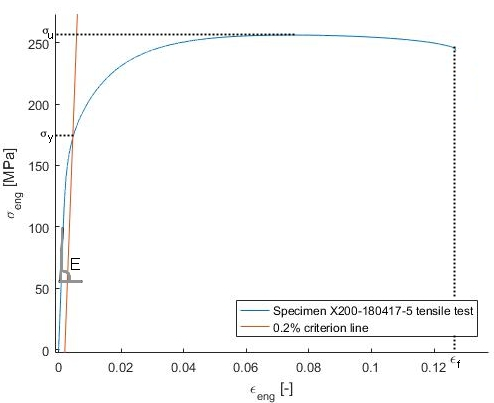
\includegraphics[scale=0.7]{Images/Tract}}
\decoRule
\caption[Tensile stress-strain curve for specimen X200-180417-5 with annotated key features]{Tensile stress-strain curve for specimen X200-180417-5 with annotated key features}
\label{fig:Tract}
\end{figure}


%\subsubsection{Fatigue}
